
\documentclass[a4paper]{article}
\usepackage{}
\usepackage[none]{hyphenat}
\usepackage{titlesec}
\usepackage{titling}
\usepackage[margin=0.63in]{geometry}
\usepackage{graphicx}
\usepackage{wrapfig}
\usepackage{enumitem}
\usepackage[hidelinks]{hyperref}
\usepackage{array}
\newcolumntype{C}[1]{>{\centering\let\newline\\\arraybackslash\hspace{0pt}}m{#1}}
\begin{document}
	\begin{center}
		\huge{\textbf{Kiran S Patil}}
		\vspace{5pt}
		\hrule
	\end{center}
	\begin{minipage}{0.5\textwidth}
		Sharda Building,\\ 
		House No.2988,  \\
		Saraswati Nagar,\\
		Belgaum-591108,\\ 
		Karnataka \\
		Contact:- +919535413763\\
		kiran.suvas.patil@gmail.com\\
	\end{minipage}
	\begin{minipage}{0.5\textwidth}	
		\hspace{153pt}
		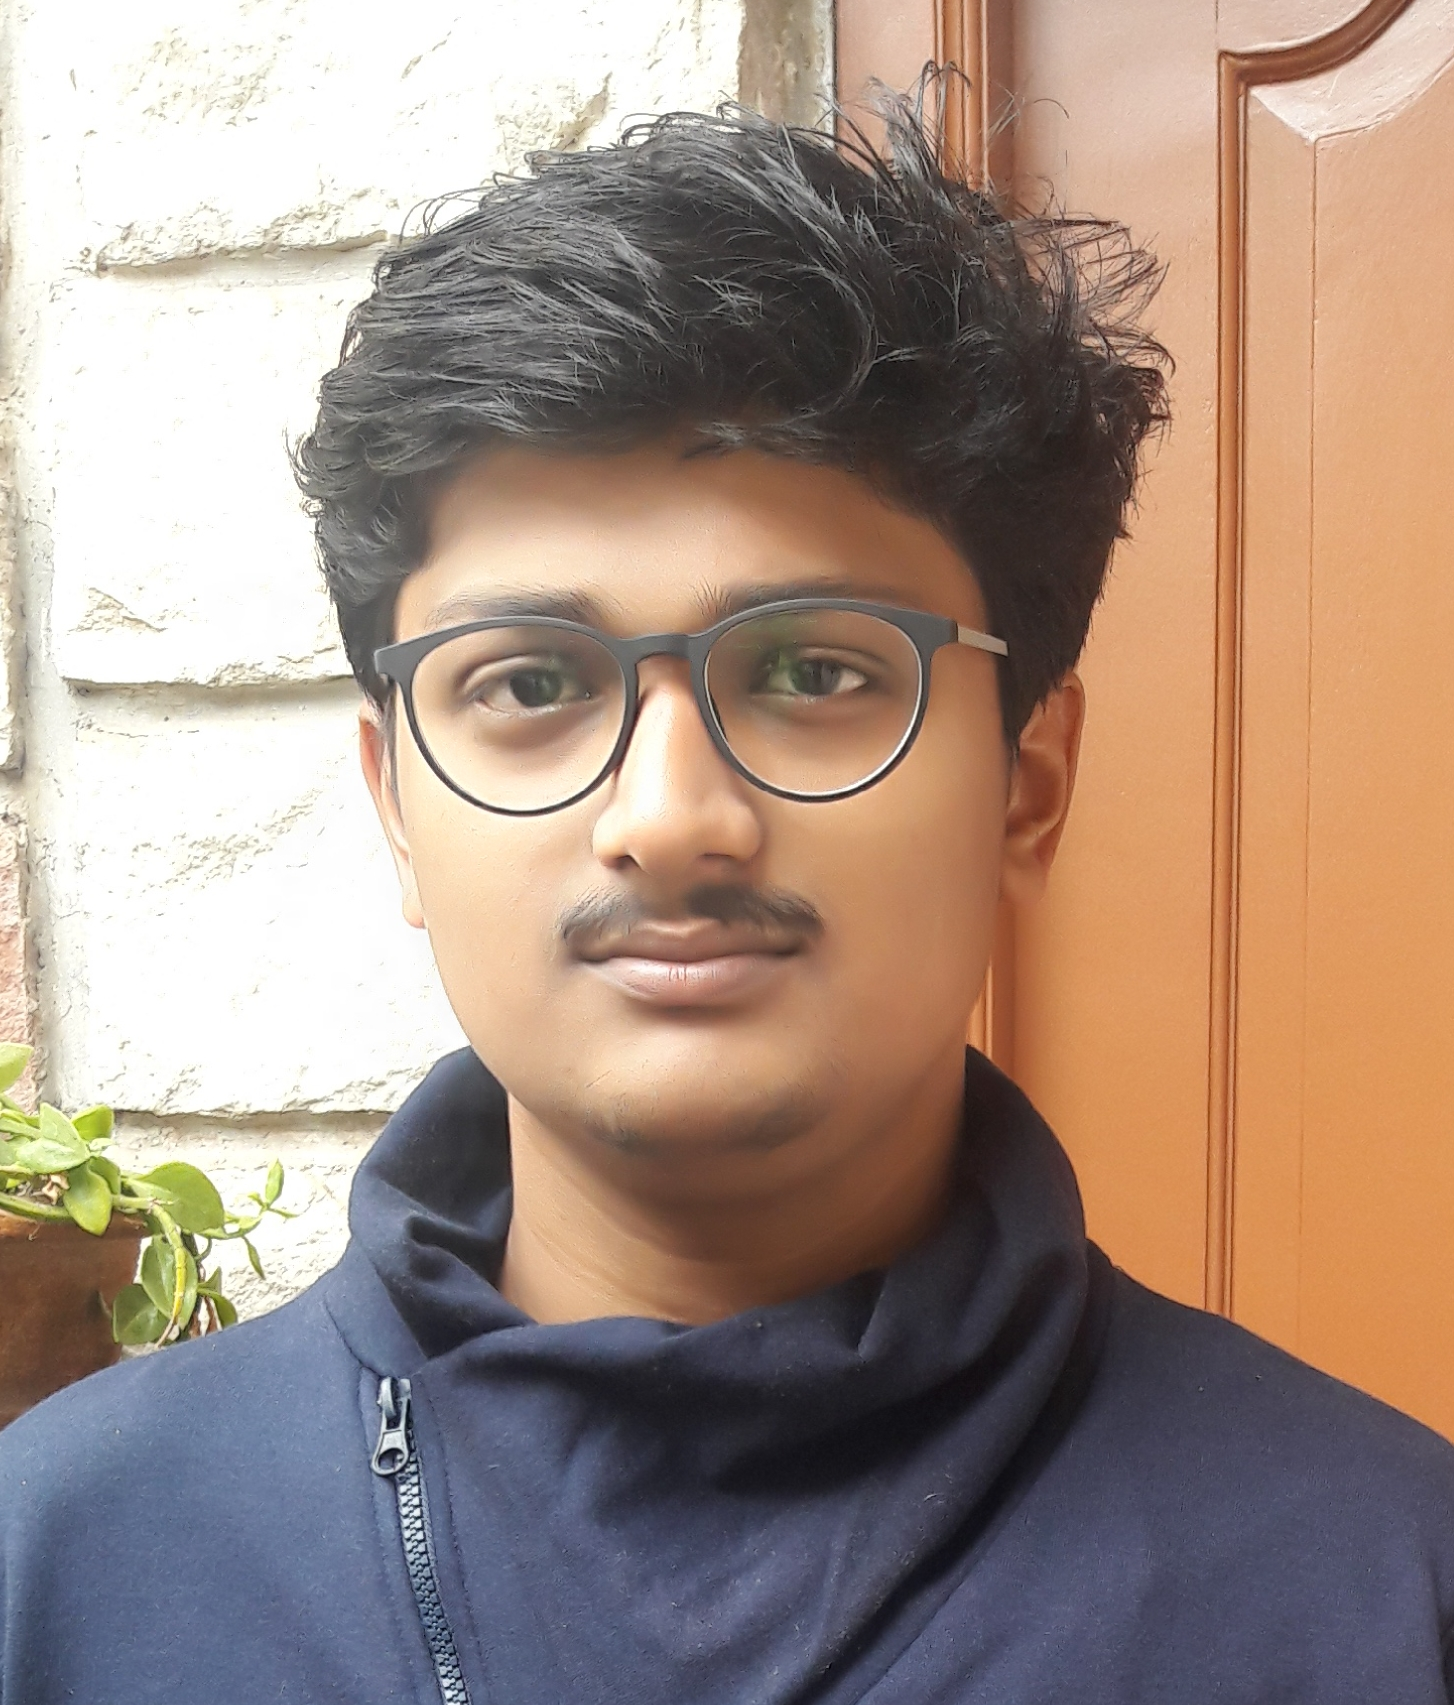
\includegraphics[scale=0.065]{image.jpg}		
	\end{minipage}

	\begin{flushleft}
		\vspace{5mm}
		\large{\textbf{OBJECTIVE}} 
		\vspace{0.5mm}
		\noindent\hrulefill
		\vspace{0.5mm}
	\end{flushleft}
	\begin{flushleft}
		An Electronics and Communication third-year undergraduate student seeking to
		pursue a career in the field of Robotics, Embedded Systems and Deep Learning.
	\end{flushleft}

	\begin{flushleft}
		\vspace{5mm}
		\large{\textbf{EDUCATION}} 
		\vspace{0.5mm}
		\noindent\hrulefill
		\vspace{0.5mm}
	\end{flushleft}
	\begin{table}[h!]
		\begin{center}
			\begin{tabular}{|C{2.4cm}|C{4.5cm}|C{4.7cm}|C{2cm}|C{2cm}|}				
				\hline \textbf{Degree} & \textbf{College/School} & \textbf{University/Board} & \textbf{Passing Year} & \textbf{Percentage}\\ \hline
				B.E (Electronics and Communication) & KLS Gogte Institute Of Technology, Belgaum & Autonomous Under Visvesvaraya Technological University & 2019 & 8.23 CGPA (1st-sem to 5th-sem)\\\hline
				12\textsuperscript{th} & Kendriya Vidyalaya No.2 Cantonment, Belgaum & Central Board of Secondary Education, Delhi & 2015 & 83.80\%\\\hline
				10\textsuperscript{th} & Kendriya Vidyalaya No.2 Cantonment, Belgaum & Central Board of Secondary Education, Delhi & 2013 & 8.4 CGPA\\\hline
			\end{tabular}
		\end{center}
	\end{table}

	\begin{flushleft}
		\vspace{5mm}
		\large{\textbf{PROJECTS}} 
		\vspace{0.5mm}
		\noindent\hrulefill
		\vspace{0.5mm}
	\end{flushleft}
	\begin{enumerate}
		\item \textbf{Harvester Bot-eYRC 2017}\\
		An autonomous robot which identifies(using image processing), plucks and deposits the required fruits on an abstract farm.  
		\item \textbf{Path finder}\\
		An autonomous robot that can traverse to its given destination even when an obstacle is introduced in its path, by managing to take an best alternative path to its destination.  
		\item \textbf{Obstacle detector}\\
		A prototype using Arduino Uno and HC-SR04(Ultrasonic sensor), which detects an obstacle/object and returns the distance.
		\item \textbf{Object Identifier}\\
		Identification of an object based on its colour and size using image acquisition technique in MATLAB.				 	              
	\end{enumerate}

	\begin{flushleft}
		\vspace{5mm}
		\large{\textbf{TRAINING \& INTERNSHIP }} 
		\vspace{0.5mm}
		\noindent\hrulefill
		\vspace{0.5mm}
	\end{flushleft}
	\begin{itemize}
		\item \href{https://blended-learning.ieee.org/BLPLMS/CL21/ProgramCertificate.aspx?ProductId=129&UserId=3148}{\textbf{RTL Design using Verilog}}\\
					Certification course under IEEE blending learning program              
	\end{itemize}

	\begin{flushleft}
		\vspace{5mm}
		\large{\textbf{RESEARCH PUBLICATIONS }} 
		\vspace{0.5mm}
		\noindent\hrulefill
		\vspace{0.5mm}
	\end{flushleft}
	\begin{enumerate}
		\item None              
	\end{enumerate}

	\begin{flushleft}
		\vspace{5mm}
		\large{\textbf{TECHNICAL SKILLS }} 
		\vspace{0.5mm}
		\noindent\hrulefill
		\vspace{0.5mm}
	\end{flushleft}
	\begin{itemize}
		\item \textbf{Programming Languages} :- C, Matlab, C++, Python, Embedded C, ARM Assembly, HTML, CSS, Verilog HDL.
		\item \textbf{Hardware Knowledge} :- Atmel ATmega 2560, Arduino, Raspberry Pi, LPC2148.
		\item \textbf{Software Knowledege} :- OpenCV, Numpy, Cadence Virtuoso, Keil uVision4, Xilinx ISE, Vivado, Multisim and Simulink.		             
	\end{itemize}

	\begin{flushleft}
		\vspace{5mm}
		\large{\textbf{SOFT SKILLS }} 
		\vspace{0.5mm}
		\noindent\hrulefill
		\vspace{0.5mm}
	\end{flushleft}
	\begin{enumerate}
		\item  Dedication, Teamwork, Persistence, Responsibility.
		\item  Languages :- Marathi, English, Hindi.        
	\end{enumerate}

	\begin{flushleft}
		\vspace{5mm}
		\large{\textbf{EXTRA-CURRICULAR ACTIVITIES }} 
		\vspace{0.5mm}
		\noindent\hrulefill
		\vspace{0.5mm}
	\end{flushleft}
	\begin{itemize}
		\item Member of Lead Cell GIT (a social innovation club at KLS GIT). 
		\item Part of a social project wherein we raised money for charity by selling lamps(diyas) during diwali. 
		\item Part of a social project wherein we donated books for setting up libraries in government schools.           
	\end{itemize}

	\begin{flushleft}
		\vspace{5mm}
		\large{\textbf{CO-CURRICULAR ACTIVITIES}} 
		\vspace{0.5mm}
		\noindent\hrulefill
		\vspace{0.5mm}
	\end{flushleft}
	\begin{enumerate}
		\item \href{http://eycgen.e-yantra.org/index.php/validate/1c554533d0991a7d96b51b2238d1d3df75ebc0b0}{\textbf{1\textsuperscript{st} Prize}\textbar National Level e-Yantra Robotics Competition (eYRC 2017),IIT Bombay\textbar Harvester Bot.}       
	\end{enumerate}

	\begin{flushleft}
		\vspace{5mm}
		\large{\textbf{PERSONAL DETAILS }} 
		\vspace{0.5mm}
		\noindent\hrulefill
		\vspace{0.5mm}
	\end{flushleft}
	\begin{itemize}
		\item \textbf{Father's Name:} Suvas K Patil
		\item \textbf{Mother's Name:} Jyotsna S Patil
		\item \textbf{Sex:} Male
		\item \textbf{Date of Birth:} 27\textsuperscript{th} August 1997
		\item \textbf{Nationality:} INDIAN
		\item \textbf{Marital Status:} Single 				          
	\end{itemize}

	\begin{flushleft}
		\vspace{5mm}
		\large{\textbf{REFERENCE}} 
		\vspace{0.5mm}
		\noindent\hrulefill
		\vspace{0.5mm}
	\end{flushleft}
	\begin{enumerate}
		\item   \textbf{Dr. Prashant P. Patavardhan}, Head of Department, Department of Electronics and Communication, KLS GIT, Belgaum\textbar +919448941840\textbar pppatavardhan@git.edu
		\item   \textbf{Prof. Supriya S. Shanbhag}, Assistant Professor, Department of Electronics and Communication, KLS GIT, Belgaum\textbar+919845306767\textbar ssshanbhag@git.edu     
	\end{enumerate}


\end{document}